\documentclass{article} % For LaTeX2e
\usepackage{iclr2016_conference,times}
\usepackage{hyperref}
\usepackage{url}
\usepackage{graphicx}
\usepackage{amsmath,amsfonts,amssymb}
\usepackage{mathtools}
\usepackage{amsthm}
\usepackage{color}

\title{\scalebox{0.95}{Unitary Evolution Recurrent Neural Networks}}


\author{Martin Arjovsky \thanks{Indicates first authors. Ordering determined by coin flip.} \\
Universidad de Buenos Aires\\
\texttt{marjovsky@dc.uba.ar} \\
\And
Amar Shah$^*$ \\
Cambridge University \\
\texttt{as793@cam.ac.uk} \\
\AND
Yoshua Bengio \\
Universit\'e de Montr\'eal, CIFAR Senior Fellow\\
\texttt{yoshua.bengio@gmail.com} \\
}

% The \author macro works with any number of authors. There are two commands
% used to separate the names and addresses of multiple authors: \And and \AND.
%
% Using \And between authors leaves it to \LaTeX{} to determine where to break
% the lines. Using \AND forces a linebreak at that point. So, if \LaTeX{}
% puts 3 of 4 authors names on the first line, and the last on the second
% line, try using \AND instead of \And before the third author name.

\newcommand{\fix}{\marginpar{FIX}}
\newcommand{\new}{\marginpar{NEW}}
\newcommand{\matr}[1]{\mathbf{#1}}
\newcommand\RR{\mathbb{R}}
\newcommand\CC{\mathbb{C}}
\newtheorem{lemma}{Lemma}
\newcommand\norm[1]{\left\lVert#1\right\rVert}
%\iclrfinalcopy % Uncomment for camera-ready version

\begin{document}


\maketitle

\begin{abstract}
Recurrent neural networks (RNNs) are notoriously difficult to train. When the eigenvalues of the hidden to hidden weight matrix
deviate from absolute value 1, optimization becomes difficult due to the well studied issue of {\it{vanishing}} and {\it{exploding}} gradients, especially when trying to learn long-term dependencies.
To circumvent this problem, we propose a new architecture that learns a unitary weight matrix, with eigenvalues
of absolute value exactly 1. We construct an expressive unitary weight matrix by composing several structured matrices that act
as building blocks with parameters to be learned. Optimization of this parameterization becomes feasible only when considering hidden
states in the complex domain. We demonstrate the potential of this architecture by achieving state of the art in several hard tasks
involving very long-term dependencies.

\end{abstract}


\section{Introduction}

Deep Neural Networks have shown increasingly good performance on a wide range of real life problems including speech recognition \citep{Hinton2012}, image recognition \citep{Krizhevsky2012} and natural language processing \citep{Collobert2011}. However, training very deep models is still a difficult task, and it becomes increasingly difficult as depth is increased. The main issue that surrounds the challenges of training deep networks is the {\it{vanishing}} and {\it{exploding}} gradients problems described in \cite{Yoshua94}. The {\it{exploding}} gradient problem results in poor optimization, while the {\it{vanishing}} gradient problem results in learning effectively only the last layers of the network.

There has been support in recent literature for using orthogonal weight matrices to help optimization \citep{Saxe2014} \citep{Quoc2015}.Orthogonal matrices have the property that they are norm preserving (i.e. $\| \matr{W} h \|_2 = \| h \|_2$). This means that you can multiply a vector with orthogonal matrices for as long as you want, without the norm of the vector blowing up or shrinking. In fact, let $h_T$ and $h_t$ be the hidden unit vectors for hidden layers $T$ and $t$ respectively, with $T >> t$ (for example with $T$ the final layer). If $C$ is the cost we are trying to minimize, then the {\it{vanishing}} and {\it{exploding}} gradient problems refer to the decay or growth of $\frac{\partial C}{\partial h_t}$ as the amount of layers increases (meaning $T \to \infty$). If

\begin{equation}
  z_{t+1} = \matr{W}_t h_t + \matr{V}_t x_{t+1}
\end{equation}
\begin{equation}
  h_{t+1} = \sigma (z_{t+1})
\end{equation}

then it's easy to show by the chain rule
\begin{equation}
  \frac{\partial C}{\partial h_t} = \frac{\partial C}{\partial h_T} \frac{\partial h_T}{\partial h_t} = \frac{\partial C}{\partial h_T} \prod_{k=t}^{T-1} \frac{\partial h_{k+1}}{\partial h_k} = \frac{\partial C}{\partial h_T} \prod_{k=t}^{T-1} \matr{D}_{k+1} \matr{W}_k^T
\end{equation}

Where $\matr{D}_{k+1} = diag(\sigma'(z_{k+1}))$ is the Jacobian matrix of the nonlinearity. Since the nonlinearity is evaluated pointwise, this Jacobian matrix is clearly diagonal.

In the following we will use the norm of a matrix to mean the spectral radius (i. e. operator 2-norm) and the norm of a vector to mean $L_2$-norm. It's good to remember that with these norms, for any matrices $\matr{A}, \matr{B}$ and vector $v$ we have by definition $\norm{\matr{A}v} \leq \norm{\matr{A}} \norm{v}$ and $\norm{\matr{A}\matr{B}} \leq \norm{\matr{A}} \norm{\matr{B}}$.

If the weight matrices $\matr{W}_k$ are norm preserving (i.e. orthogonal or unitary), then we can {\bf{prove}}
\begin{equation}
  \norm{ \frac{\partial C}{\partial h_t} } = \norm{ \frac{\partial C}{\partial h_T} \prod_{k=t}^{T-1} \matr{D}_{k+1} \matr{W}_k^T } \leq \norm{\frac{\partial C}{\partial h_T}} \prod_{k=t}^{T-1} \norm{ \matr{D}_{k+1} \matr{W}_k^T } = \norm{ \frac{\partial C}{\partial h_T}} \prod_{k=t}^{T-1} \norm{\matr{D}_{k+1}}
\end{equation}

Since $\matr{D}_k$ is diagonal, then $\norm{\matr{D}_k} = \max_{j=1, ..., n} |\sigma'(h_k^{(j)})|$, with $h_k^{(j)}$ the $j$-th unit of the $k$-th hidden layer.

If the absolute value of the derivative $\sigma'$ can be some number $\lambda > 1$, then this bound is useless, because it results on $\norm{\frac{\partial C}{\partial h_t}} \leq \norm{\frac{\partial C}{\partial h_T}} \lambda^{T-t}$ which grows {\it{exponentially}} with $T-t$. This means that we cannot effectively bound $\frac{\partial C}{\partial h_t}$ for deep networks, potentially resulting in {\it{exploding}} gradients.

Even worse would be the case where $|\sigma'| < \lambda < 1$, because we would be proving that $\frac{\partial C}{\partial h_t}$ goes exponentially to 0, resulting in certain vanishing gradients. With this argument, the rectified linear unit (ReLU) \citep{Glorot2011} \citep{Nair2010} nonlinearity arises naturally. Unless all the activations are killed at one layer (which has never been reported), the maximum entry of $\matr{D}_k$ will be 1, leading to $\norm{\matr{D}_k} = 1$ for all layers $k$. With this, we effectively prove that
\begin{equation}
  \norm{\frac{\partial C}{\partial h_t}} \leq \norm{ \frac{\partial C}{\partial h_T}} \prod_{k=t}^{T-1} \norm{\matr{D}_{k+1}} = \norm{\frac{\partial C}{\partial h_T}}
\end{equation}

What is most important is the fact that this result is independent from the deep of the network or $T-t$. For the case of recurrent networks, it's easy to show that this results on the fact that $\frac{ \partial C}{\partial \theta}$ can grow at most {\it{additively}} instead of exploding {\it{multiplicatively}}. Among other things, this implies that the use of gradient clipping \citep{Pascanu2013} is no longer required.

To the best of our knowledge, this is the first time a deep neural network has been mathematically proven to have no exploding gradients.

%Notes: 
%
%- Vanishing and exploding gradients.
%
%- Support for orthogonal matrices. Results of Quoc's stuff with orthogonality.
%
%- Prove lower bound for orthogonal matrices up to jacobian matrix norms.
%
%- Introduce ReLUs as a natural solution to norm of D to be 1. Support for relus, why orthogonality + relus make sense (additive growth at most).
%
%- 

\section{Unitary Evolution RNNs}

The most important feature of unitary and orthogonal matrices for our purpose is that they have eigenvalues $\lambda_j$ with absolute value 1 (we therefore write $\lambda_j = e^{i w_j}$ with $w_j \in \RR$). A naive method to learn a unitary matrix would be to fix a basis of eigenvectors $\matr{V} \in \mathbb{C}^{n \times n}$ and set

$$ \matr{W} = \matr{V} \matr{D} \matr{V}^{*} $$

where $\matr{D}$ is a diagonal such that $\matr{D}_{j,j} = e^{i w_j}$. By restricting the choice of $\matr{V}$ and tying the learned $w_j$s to create conjugates, $\matr{W}$ can be restricted to be a real matrix. This is evident from the following lemma:

\begin{lemma}
  A complex square matrix $\matr{W}$ is unitary if and only if it has an eigendecomposition of the form $\matr{W} = \matr{V} \matr{D} \matr{V}^*$. Here, $\matr{V}, \matr{D} \in \mathbb{C}^{n \times n}$ are complex matrices, where $\matr{V}$ is unitary, and $\matr{D}$ is a diagonal such that $|\matr{D}_{j,j}|=1$. Furthermore, $\matr{W}$ is a real orthogonal matrix if and only if for every eigenvalue $\matr{D}_{j,j} = \lambda_j$ with eigenvector $v_j$, there is also an eigenvalue $\lambda_k = \overline{\lambda_j}$ with corresponding eigenvector $v_k = \overline{v_j}$
\end{lemma}
\begin{proof}
  See \cite{linalgbook}
\end{proof}

To achieve a real orthogonal matrix $\matr{W}$ we require a fixed unitary matrix $\matr{V}$, whose columns come in complex conjugate pairs $v_k = \overline{v_j}$. Similarly, we should also tie $w_k=-w_j$ in order to achieve $e^{i w_j} = \overline{e^{i w_k}}$. $\matr{W}$ is subsequently real and orthogonal by the lemma. Since $w_j$ are real numbers and if the cost is differentiable with respect to them, we can learn these weights by gradient descent. 

However, this approach has one major problem. Mainly, the memory needed to store $\matr{V}$ is $\mathcal{O}\left(n^2\right)$. Also, if $u$ is a vector, calculating $\matr{V}u$ has cost $\mathcal{O}\left( n^2 \right)$. This would lead to a cost of $\mathcal{O} \left( n^2 \right)$ for forward and backpropagation. However, we are only learning $\mathcal{O}(n)$ parameters, which is very inefficient.

If we didn't have $\matr{V}$ then we would just be learning a diagonal matrix, which likely isn't sufficient. However, since the product of unitary matrices is itself unitary, we can construct $\matr{W}$ by combining several simple structured unitary matrices that are efficient to store and to operate with. \cite{dfc} do a similar construction to reduce the amount of parameters by more than an order of magnitude in an industrial sized network, while maintaining performance. This, combined with earlier work by \cite{fastfood} suggests that it is possible to create very expressive matrices with relatively little cost. The building blocks we use are as follows:

\begin{itemize}
  \item $\matr{D}$ is a diagonal matrix with entries $\matr{D}_{j,j} = e^{i w_j}$ Since $\matr{D}$ is a diagonal with that have absolute value 1, it is clearly unitary. The weights $w_j \in \RR$ are going to be learned by gradient descent.
  \item $\matr{R} = \matr{I} - 2 \frac{v v^*}{\|v\|^2}$ is a reflection matrix by the complex vector $v \in \mathbb{C}^n$. This matrix is also learned, by doing gradient descent on the real and imaginary parts of $v$. The fact that this matrix is unitary is left as an exercise to the reader.
  \item $\matr{\Pi}$ a fixed random permutation. Since the transpose is the inverse permutation, the unitary condition follows.
  \item $\mathcal{F}$ and $\mathcal{F}^{-1}$ the Fourier and inverse Fourier transforms, which have long been showed to be unitary.
\end{itemize}

For the case of $\matr{D}, \matr{R}, \matr{\Pi}$, storing each of this matrices has cost $\mathcal{O}(n)$. For the diagonal, we only store the weights $w_j$, for the reflection only the vector $v$ and for the permutation we save it as an array. Multiplying any of this matrices with a vector is also $\mathcal{O}(n)$. The Fourier transforms don't need to be stored, and multiplying a vector with them can be done in $\mathcal{O}(n \log n)$ via the Fast Fourier Transform. This means that the final cost of doing forward and backpropagation through the weight matrix is $\mathcal{O} (n \log n)$, with memory cost $\mathcal{O} (n)$ with $\mathcal{O}(n)$ parameters and hidden units.

One major advantage of this parameterization, is that the number of parameters, memory and computational cost increase linearly as a function of the hidden layer size. Therefore, we can potentially have inmense hidden layers, while this would be impossible in traditional RNNs. Especially for modelling long term dependencies, this is not a minor feature, because it increases the amount of information that can be carried from one time to another. Early work by \cite{Yoshua94} shows that having a big memory may be a crucial aspect of solving the difficulties in modeling long-term dependencies.

We call any architecture that uses a unitary hidden to hidden matrix a unitary evolution RNN (uRNN). After trying different combinations, the uRNN we settled on has the weight matrix

$$ \matr{W} = \matr{D_3} \matr{R_2} \mathcal{F}^{-1} \matr{D}_2 \matr{\Pi} \matr{R_1} \mathcal{F} \matr{D}_1 $$

The main issue of most of this matrices (except the permutation) is that they are complex. However, they are parameterized with real weights, so if the final cost is real and is differentiable with respect to them, we can do gradient descent nonetheless. In the following section we specify the complete architecture of the network, and explain how the potential difficulties of using complex hidden units can be easilly bypassed.

\section{Architecture details}

It is not enough to say how to parameterize a unitary weight matrix and get done with it. In this section, we describe the rest of the architecture, including the nonlinearity we used, how we go from real input to complex hidden units and from these units to the output.

\subsection{Complex hidden units}

All the hidden units are represented internally with real numbers, as imaginary and complex parts. This way, it is far more easy to code, and we completely avoid the lack of support for complex numbers by most deep learning frameworks. One of the most important examples is when multiplying the weight matrix $\matr{W} = \matr{A} + i \matr{B}$ by the complex hidden vector $h = x + i y$ In fact, it is easy to show that $ \matr{W}h = (\matr{A}x - \matr{B}y) + i (\matr{A}y + \matr{B}x) $, which leads to


$$ \begin{pmatrix} Re(\matr{W}h) \\ Im(\matr{W}h) \end{pmatrix}  = \begin{pmatrix} \matr{A} & -\matr{B} \\ \matr{B} & \ \ \ \matr{A} \end{pmatrix} \begin{pmatrix} Re(h) \\ Im(h) \end{pmatrix}$$

More generally, let $f: \CC^n \rightarrow \CC^n$ be any complex function and $z = x + i y$ any complex vector, it can be decompposed as $ f(z) = u(x, y) + i v(x, y) $ where $u,v$ are the real and imaginary parts of $f$. Therefore, we can consider the mapping as $f: \RR^{2n}  \rightarrow \RR^{2n}$, and implement everything with real numbers. Doing this, any Deep Learning framework with automatic differentiation like Theano \citep{Fred2010} is able to take care of computing the derivatives efficiently.

\subsection{Input to hidden and the nonlinearity}

As is the case with most recurrent networks, our uRNN follows the same hidden to hidden mapping as equation (1) with $\matr{V}_t = \matr{V}$ and $\matr{W}_t = \matr{W}$. For the input matrix we have $\matr{V} \in \CC^{n \times n}$, and it's real and imaginary. The initial hidden state $h_0 \in \CC^n$ is learned this way as well.

Sadly, it is not as easy to choose a good nonlinearity. As discussed in section 1, using a ReLU is the natural choice when having an orthogonal or unitary RNN. Previous work on complex RNNs usually have applied a nonlinearity on both the real and imaginary parts \ref{Old CRNN papers}. However, as we will show later, this usually results on poor performance. The interpetation of why this happens is that applying a nonlinearity on the real and imaginary parts brutally changes the phase of a complex number. Since unitary matrices can be interpreted as multiplying by a phase in each eigenvector direction, this phase might be important when recovering information about past memories. Therefore, we employ a variation of the ReLU that we deem modReLU, that is applied only on the absolute value, and is defined as follows.

$$ \sigma: \CC \rightarrow \CC $$

$$ \sigma (z) = 
\left\{
  \begin{array}{ll}
    (|z|+b|) \frac{z}{|z|}  & \mbox{if } |z| + b \geq 0 \\
    0 & \mbox{if } |z| + b < 0
  \end{array}
\right.
$$


Where $b \in \RR$ is the bias of the nonlinearity, which is learned for each complex unit. It is important to note that $\sigma(z) = \text{ReLU}(|z| + b) \frac{z}{|z|}$

\subsection{Hidden to output}

For the output we have a matrix $\matr{U} \in \RR^{2n_h \times n_o}$ where $n_h$ is the hidden layer size and $n_o$ is the output size. The output is calculated as

$$ o_t = \matr{U} \begin{pmatrix} Re(h_t) \\ Im(h_t) \end{pmatrix} + b_o $$

with $b_o \in \RR^{n_o}$ the output bias. Since this output is real, we can now use it to compare the cost in the classical way with any loss function (e.g. plug it into a softmax for classification).
\subsection{Initialization}

We experimented with several initialization strategies. However, because of the stability of the network, initialization doesn't seem to be extremely important. However, the following ones did seem to make optimization marginally easier, and give a few insights on the way the netwrok works.

\begin{itemize}
  \item We initialize $\matr{V}$ and $\matr{U}$ (the input and output matrices) as in \cite{Glorotinit} with a uniform $\mathcal{U}\left[-\frac{\sqrt{6}}{\sqrt{n_{in}+ n_{out}}}, \frac{\sqrt{6}}{\sqrt{n_{in}+ n_{out}}}\right]$.
  \item The biases are initialized to 0. This way at the beginning, the nonlinearity is silent. This is because the input of the ReLU is always positive (it is an absolute value). Therefore, we start with a linear unitary mapping with additive contributions from the input, which is controled and seems to help early optimization \citep{Quoc2015}.
  \item The reflection vectors for $\matr{R}_1$ and $\matr{R}_2$ are initialized coordinate-wise from a uniform $\mathcal{U}[-1, 1]$. It's important to remark the fact that since the reflection matrix is independent from the scale of the vector, so any centered uniform will result in the same network.
  \item The diagonal weights $w_j$ are sampled from a uniform $\mathcal{U}[-\pi, \pi]$. This way $\matr{D}_{j,j} = e^{i w_j}$ is sampled uniformly from the unit circle.
  \item We initialize $h_0$ with a uniform $\mathcal{U}\left[-\sqrt{\frac{3}{2n_h}}, \sqrt{\frac{3}{2n_h}} \right]$. This way $\mathbb{E}\left[\|h_0\|^2\right] = 1$. Since the norm of the hidden units is roughly preserved because of the unitary weight matrix and inputs are usually whitened to have norm 1, we have hidden states and inputs on the same order of magnitude, which seems to help optimization \ref{batchnorm?}.
\end{itemize}

\section{Experiments}
In this section we show the performance of our uRNN on several tasks related to learning long-term dependencies. These problems were especially created to be pathologically hard, and have been used as benchmarks for testing the capacity of a model to capture long-term memory \citep{LSTM} \citep{HF} \citep{Quoc2015}.

\subsection{Copying memory problem}
Recurrent networks have major issues when the outputs they try to model depend on inputs that were sent a long time ago \citep{Yoshua94} \citep{Pascanu2013}. Therefore, it is a natural task to ask a recurrent network to reproduce exactly an input it has seen long ago.

The task starts with the network being fed 10 symbols choosen uniformly at random between $\{a_i\}_{i=0}^7$ and represent the sequence to be remembered. Then we give the network another symbol $a_8$ repeated for a very long time. We give this symbol $a_8$ the name `blank'. After the repeated blanks, the network reads the symbol $a_9$, followed again by blanks. This is the precise moment when the network is supposed to start outputing the 10 original symbols. At any other time, the network should ouput blanks.
If the entire input sequence has length $T$, the effective time lag for which our network needs to remember the symbols is $T-10$. When $T$ is long enough, this problem becomes violently hard for current approaches.

A baseline can be established by realizing what the best strategy is without remembering any of the 10-digit input. This strategy (which we deem memory-less) would be to predict a blank at every position except for the ten outputs after the delimiter $a_9$, and in those position uniformly at random from $\{a_i\}_{i=0}^7$. Since we are using cross-entropy, if $o_t$ is the probability that the network outputs for the correct answer at time $t$ then the cost of this strategy is exactly

\begin{equation}
  -\frac{\sum_{t=1}^{T+20} \log (o_t)}{T+20} = - \frac{\sum_{t=T+11}^{T+20} \log \left( \frac{1}{8} \right)}{T+20} = \frac{10 \log(8)}{T+20} 
\end{equation}

\begin{figure}[ht] 
  \label{ fig7} 
  \begin{minipage}[b]{0.5\linewidth}
    \centering
    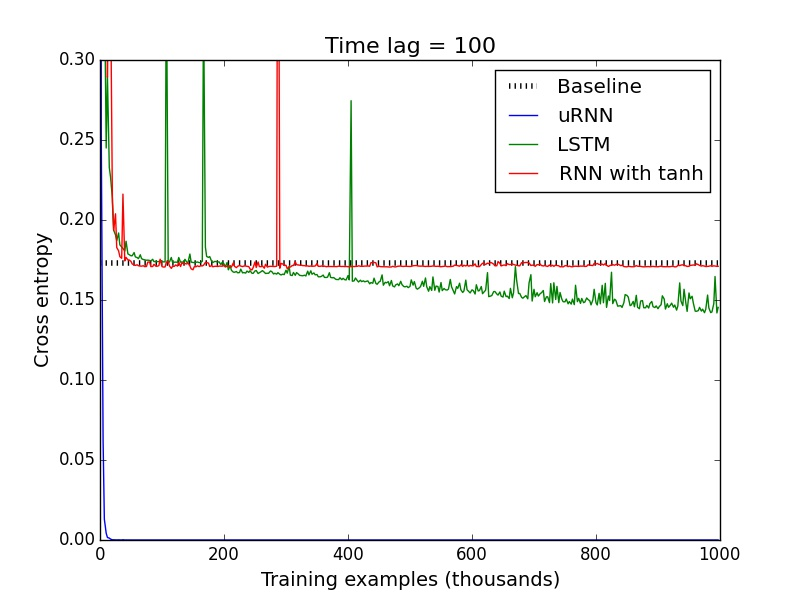
\includegraphics[scale=0.25]{figures/memory_100.jpeg}
    \vspace{4ex}
  \end{minipage}%%
  \begin{minipage}[b]{0.5\linewidth}
    \centering
    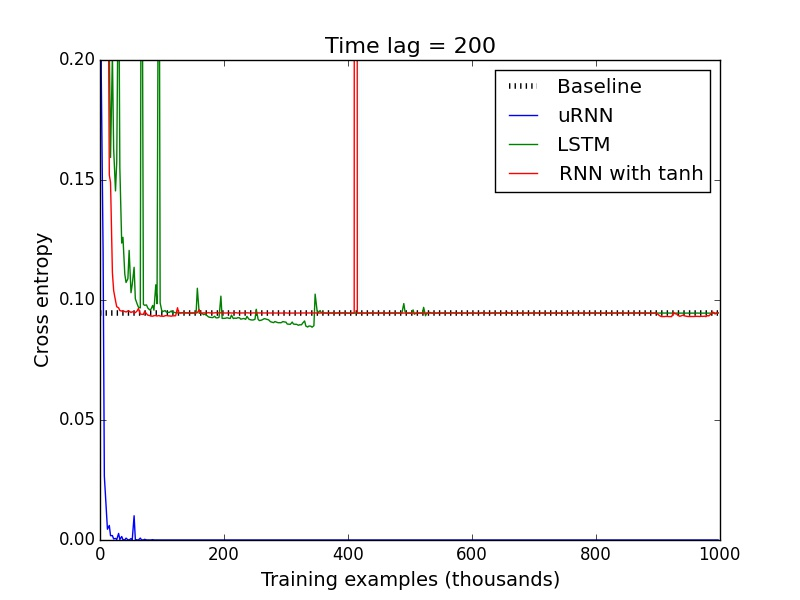
\includegraphics[scale=0.25]{figures/memory_200.jpeg}
    \vspace{4ex}
    \end{minipage} 
  \begin{minipage}[b]{0.5\linewidth}
    \centering
    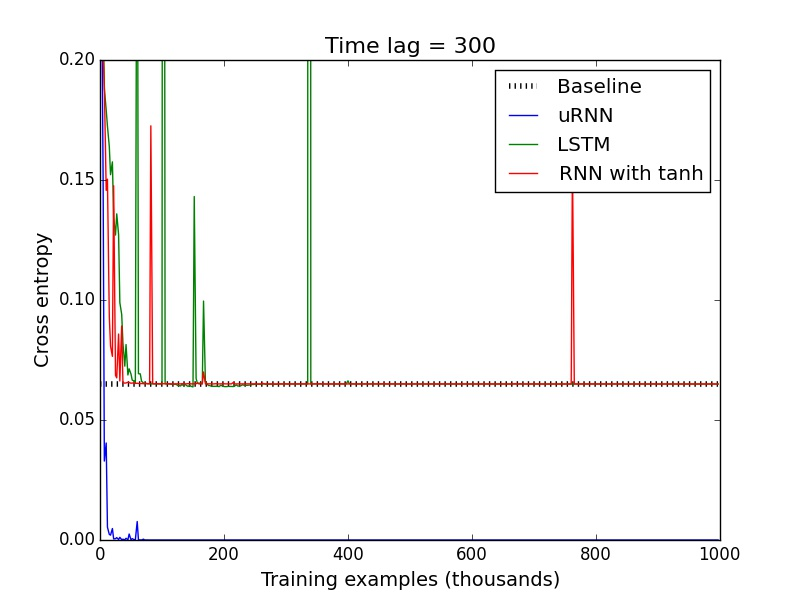
\includegraphics[scale=0.25]{figures/memory_300.jpeg}
    \vspace{4ex}
    \end{minipage}%% 
  \begin{minipage}[b]{0.5\linewidth}
    \centering
    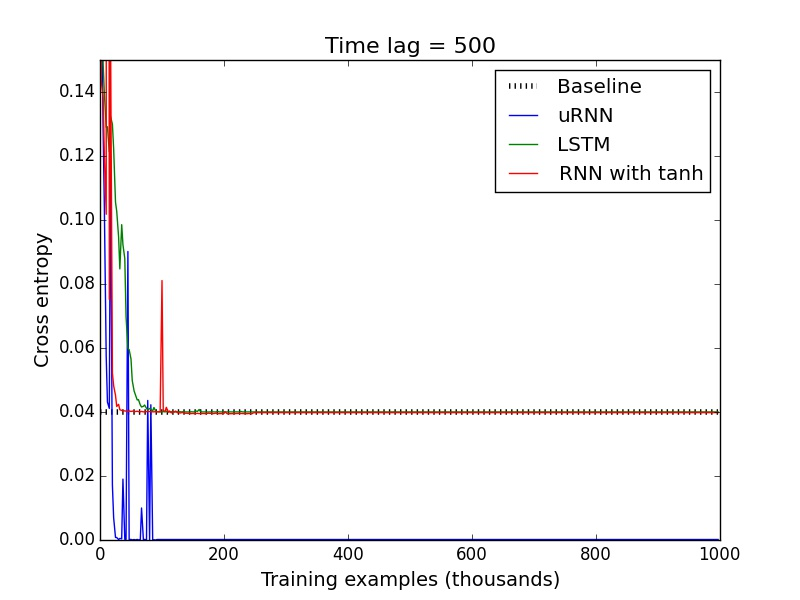
\includegraphics[scale=0.25]{figures/memory_500.jpeg}
    \vspace{4ex}
  \end{minipage} 
\end{figure}

We ran these experiments for an RNN with tanh activations, an LSTM and an IRNN to compare with our uRNN. All networks except the uRNN have 32 hidden units. This results in about 1000 parameters for the RNN and IRNN, and 4000 for the LSTM. The uRNN was run with 128 hidden units, or about 1900 parameters (less than half as the LSTM). All experiments where done using RMSPROP \citep{RMSPROP}. The IRNN was extremely unstable throughout the experimentation, and we could avoid divergence only with a delay of 100 and learning rate of $10^{-8}$. Because of this, it is not included in the figures, and the plot for this IRNN is shown in the appendix.

In figure 1, we see that except in the simplest case both the RNN with tanh and more surprisingly the LSTMs get almost exactly the same cost as the memoryless strategy. This behaviour is consistent with the results of \cite{NTM}, in which poor performance is evidenced by LSTMs for a very similar problem.

What is very interesting is not only the fact that the uRNN displays perfect performance in very little iterations, but how qualitatively different the results are from the LSTM. One of the most noticeable features is that it goes from initialization to almost 0 cost without staying at the baseline. In contrast, for the first plot, the LSTM stays on the baseline for a while, before starting to improve very slowly. This evidences the fact that the uRNN is a very different model than both LSTMs and classical RNNs, potentially achieving very different internal representations.

\subsection{Adding Problem}
In this problem, the input consists of two sequences of length $T$. The first sequence (let's call it $x$) consists of numbers sampled uniformly at random from a uniform $\mathcal{U}[0,1]$. The second one consists of all zeros, except for two positions that are 1. This two positions (let's call them $i$ and $j$) are sampled at random from the first and second half respectively. An output is given only after the last time step, and it is $x_i + x_j$ (i.e. the numbers from the first sequence in the marked positions).

\begin{figure}[ht] 
  \label{ fig7} 
  \begin{minipage}[b]{0.5\linewidth}
    \centering
    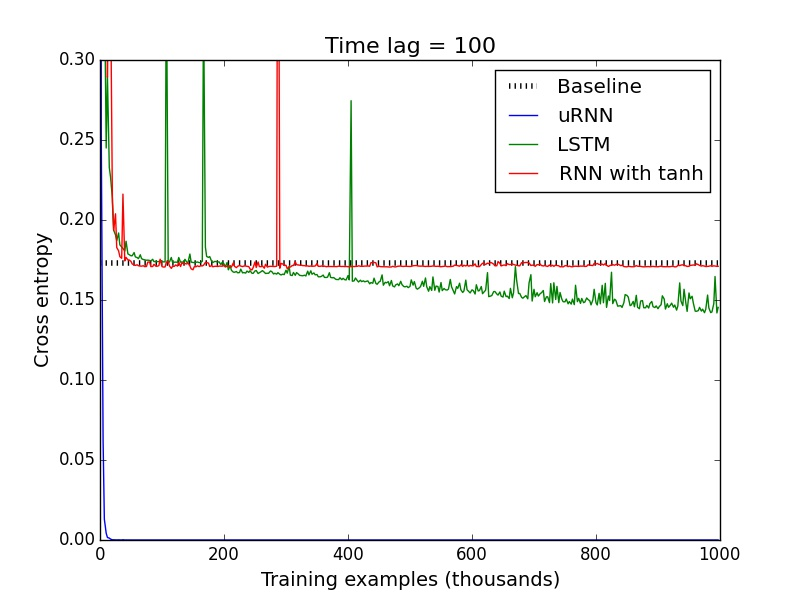
\includegraphics[scale=0.25]{figures/memory_100.jpeg}
    \vspace{4ex}
  \end{minipage}%%
  \begin{minipage}[b]{0.5\linewidth}
    \centering
    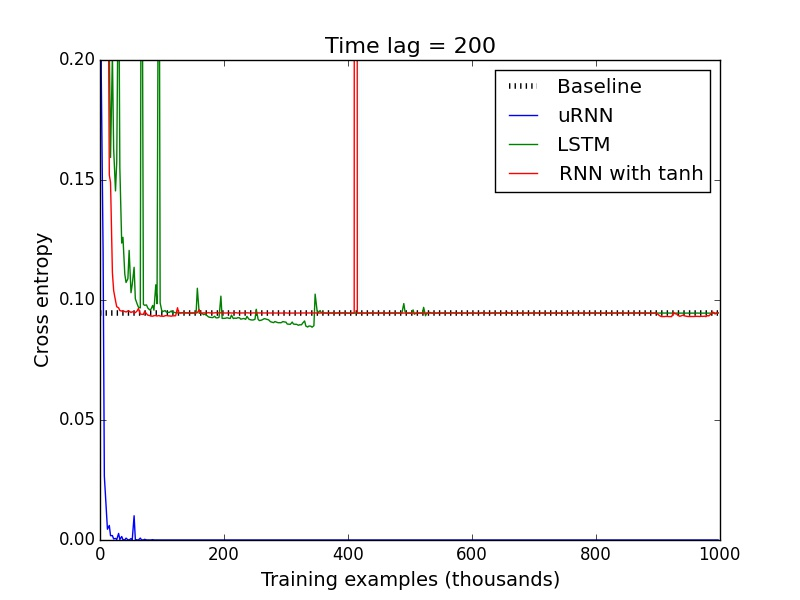
\includegraphics[scale=0.25]{figures/memory_200.jpeg}
    \vspace{4ex}
    \end{minipage} 
  \begin{minipage}[b]{0.5\linewidth}
    \centering
    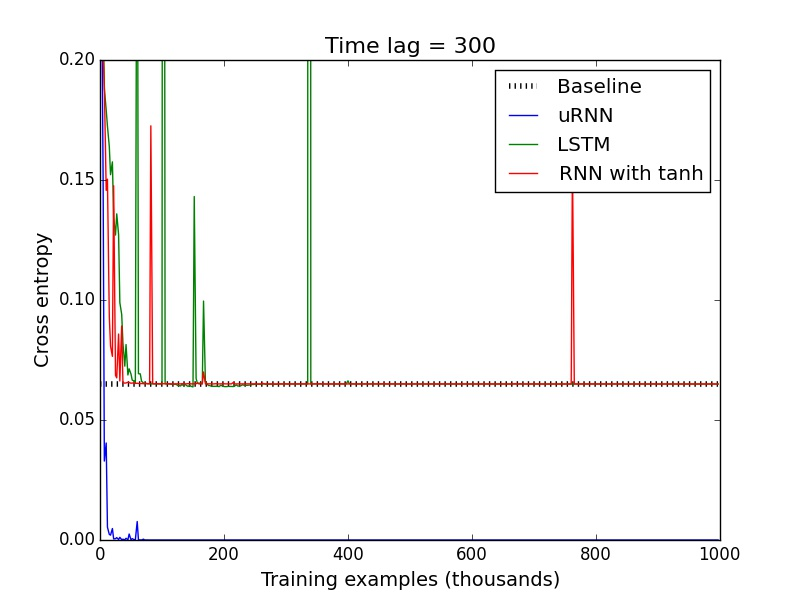
\includegraphics[scale=0.25]{figures/memory_300.jpeg}
    \vspace{4ex}
    \end{minipage}%% 
  \begin{minipage}[b]{0.5\linewidth}
    \centering
    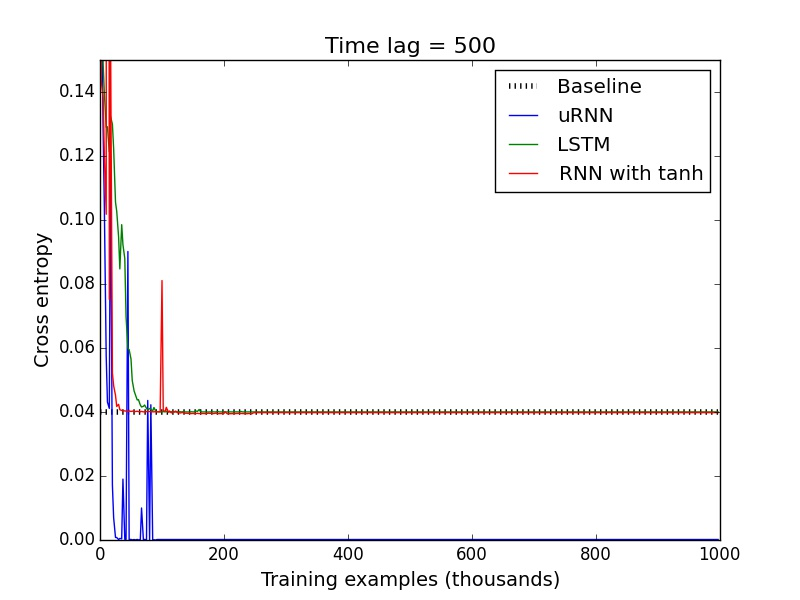
\includegraphics[scale=0.25]{figures/memory_500.jpeg}
    \vspace{4ex}
  \end{minipage} 
\end{figure}


\subsection{Pixel-by-pixel MNIST}
IRNN

\subsection{Optimization experiments}
Ian Good

\bibliography{uRNN}
\bibliographystyle{uRNN}

\end{document}
